\documentclass[11pt, oneside]{article}
\usepackage{geometry}
\geometry{letterpaper, margin=0.8in,top=0.75in}
\usepackage[utf8]{inputenc}
\usepackage[english]{babel}

\usepackage{amsmath}
\usepackage{amssymb}
\usepackage{amsthm}
\usepackage[ruled,vlined]{algorithm2e}
\usepackage{graphicx}
\usepackage{siunitx}
\usepackage{booktabs}
\usepackage{array}
\usepackage{subcaption}

\title{MCSC 6020G - Numerical Analysis \\
        \Large Assignment 2}
\author{Parikshit Bajpai}
\date{}

\newtheorem*{remark}{To prove}
\newtheorem*{order}{Complexity}
\renewcommand\qedsymbol{$\blacksquare$}

\begin{document}
\maketitle

\section*{Question 1}
	\begin{remark}
		Every strictly column diagonally dominant matrix $A \in \mathbb{C}^{n \times n}$ is nonsingular. 
	\end{remark}
	\begin{proof}
		A matrix $A \in \mathbb{C}^{n \times n}$ is strictly column diagonally dominant if 
		\begin{equation}\label{eq:cdd}
			|a_{j,j}| > \sum_{i=1, i\neq j}^n |a_{i,j}|
		\end{equation}
		
		Consider the transpose of matrix $A$, $A^T \text{ whose elements} a^T_{ij} a_{ji}$. Then, from equation~\eqref{eq:cdd}:
		\begin{equation}\label{eq:cdd}
			|a_{j,j}| >  \sum_{i=1, i\neq j}^n |a_{i,j}| = \sum_{j=1, i\neq j}^n |a^T_{i,j}|
		\end{equation}
		i.e., $A^T$ is strictly row diagonally dominant.  
		
		Strictly row diagonally dominant matrix $A^T \in \mathbb{C}^{n \times n}$ can be decomposed into a diagonal matrix $D$ whose elements are $a^T_{ii}$ and matrix $B$ with diagonal elements equal to zero. It's non-singularity can then be shown as follows:
		\begin{align}
			|a_{j,j}| > \sum_{i=1, i\neq j}^n |a_{i,j}|\\
			1 > \frac{1}{|a_{j,j}|} \sum_{i=1, i\neq j}^n |a_{i,j}|
		\end{align}
		The second inequality is equivalent to: 
		\begin{align} \label{eq:contra1}
			1 > \|D^{-1} B\|_{\infty}
		\end{align}
		
		If $A^T$ was singular, $\exists x \neq 0$, such that $A^Tx=0$.
		\begin{align}
			A^Tx = 0 \\
			(D + B)x = 0\\
			x = D^{-1} B x
		\end{align}
		
		Using infinity norm:
		\begin{equation}
			\|x\|_{\infty}  =   \|D^{-1} B x \|_{\infty} \leq \|D^{-1} B\|_{\infty} \|x \|_{\infty}
		\end{equation}
		
		Dividing by $\|x\|_{\infty}$
		\begin{equation}
			1 \leq   \|D^{-1} B \|_{\infty} 
		\end{equation}
		
		This contradicts equation~\eqref{eq:contra1} and hence every strictly row diagonally dominant must be non singular.
		 
		Non-singularity of strictly row diagonally dominant $A^T$ implies $det(A^T) \neq 0$. Since $det(A^T) = det(A)$, $det(A) \neq 0$, i.e., $A$ is non-singular. 	
	\end{proof}

\section*{Question 2}
\subsection*{(a) 2 norm of a square matrix}
  	\begin{remark}
    		For a matrix $A \in \mathbb{C}^{n \times n}$ given by the outer product $A = y x^T$, $\|A\|_2 = \|x\|_2 \|y\|_2$.
  	\end{remark}
	
  	\begin{proof} For a matrix $A \in  \mathbb{C}^{n \times n}$,
    		\begin{align}
    			\|A\|_2 &= \max_{v \in \mathbb{C}^{n \times n}} \frac{\|Av\|_2}{\|v\|_2} \\
				&= \max_{v \in \mathbb{C}^{n \times n}} \frac{\|yx^Tv\|_2}{\|v\|_2} && \left(\because A = yx^T \right) \\
				&= \max_{v \in \mathbb{C}^{n \times n}} \frac{|x^Tv|\|y\|_2}{\|v\|_2} \\
				&= \max_{v \in \mathbb{C}^{n \times n}} \frac{|x^Tx|\|y\|_2}{\|x\|_2} && \left(\text{Take } v = x\right) \\
				&= \frac{\|x\|_2\|x\|_2 \|y\|_2}{\|x\|_2} && \left(\text{Cauchy-Schwarz, } |uv| \leq \|u\|_2\|v\|_2, \text{ equality holds if } u=v \right) \\
				&= \|x\|_2 \|y\|_2 && \qedhere
    		\end{align}
  	\end{proof}
  
\subsection*{(b) Condition number of matrix}
  	\begin{remark}
    		For invertible matrices $A \in \mathbb{C}^{n \times n}$ and $B \in \mathbb{C}^{n \times n}$, condition number $K_p(AB) \leq K_p(A) K_p(B)$, where $K_p(A) = \|A\| \|A^{-1}\|$. 
  	\end{remark}
	
  	\begin{proof} For matrix $AB \in  \mathbb{C}^{n \times n}$,
    		\begin{align}
    			K_p(AB) &= \|AB\|_p \|(AB)^{-1}\|_p \\
					&= \|AB\|_p \|B^{-1}A^{-1}\|_p && \left(\because (AB)^{-1} = B^{-1} A^{-1}\right)\\
					&\leq \|A\|_p \|B\|_p  \|B^{-1}\|_p  \|A^{-1}\|_p && \left(\because \|AB\|_p \leq  \|A\|_p \|B\|_p\right)\\
					&\leq  \left(\|A\|_p \|A^{-1}\|_p \right) \left(\|B\|_p  \|B^{-1}\|_p\right) \\
					&\leq K_p(A) K_p(B) && \qedhere
    		\end{align}
  	\end{proof}
  
\section*{Question 3}
\subsection*{(a) Monotonically decreasing convex function}
  	\begin{remark}
    		Function $f$ is a monotonically decreasing convex function on $[0,\infty)$, where $f$ is of the following form
    		\begin{equation}
    			f(x) = \sum_{i=1}^{N} \frac{a_i^2}{(b_i^2 + x)^2} \mspace{50mu} \text{For } a_i,\,b_i \in \mathbb{R}  
    		\end{equation} 
 	\end{remark}

  	\begin{proof}
		\begin{align}
			\frac{df}{dx} = -2 \sum_{i=1}^{N} \frac{a_i^2}{(b_i^2 + x)^3}  \leq 0 && \forall x \in [0,\infty) \\
			\frac{d^2f}{dx^2} = 6 \sum_{i=1}^{N} \frac{a_i^2}{(b_i^2 + x)^4}  \geq 0 && \forall x \in [0,\infty)
		\end{align}
		Since the first derivative of the function is negative in the given domain, the function is monotonically decreasing and since the second derivative is positive in the domain, the function is convex.
  	\end{proof}
  
\subsection*{(b) Newton's method}
Newton's method was implemented to find the roots of $f(x) = \delta$, where $0 < \delta < f(0)$. Since the convergence of Newton's method depends on the initial guess $x_0$, a number of ``manufactured" solutions were tested for different combinations of $a_i$, $b_i$ and $N$. Using the manufactured solutions, the implementation was verified to ensure that the algorithm works when provided with a suitable initial estimate. The different combinations used are listed in table~\ref{tab:testcases} and figure~\ref{fig:residuals_newton} shows the residuals versus the number of Newton iterations. The plots show that the Newton method converges almost quadratically once it gets close to the real root. However, if the initial guess $x_0$ is not sufficiently close to the real root, Newton method can often converge at a very slow rate or not converge at all. Since the manufactured solutions were provided with initial guesses close enough to the real roots, non-convergence was not observed. However, in a number of cases, the method showed a very slow initial progress and then once it got close enough to the final estimate the rate of convergence became close to quadratic.

	\begin{table}[htbp]
		\caption{Parameters $a_i, b_i \text{ and } N$ used in the manufactured functions. $\delta$ and  $x_0$ are also shown.}
		\centering
		\begin{tabular}{@{}m{2cm}m{1cm}m{1cm}m{1cm}m{1cm}m{1cm}m{1cm}m{1cm}m{1cm}m{1cm}m{1cm}@{}}
            		\toprule
            		\textbf{Parameters} & \textbf{Case I} & \textbf{Case II} & \textbf{Case III} & \textbf{Case IV}  & \textbf{Case V}& \textbf{Case VI}& \textbf{Case VII}& \textbf{Case VIII}& \textbf{Case IX}& \textbf{Case X}\\
            		\midrule
            		$N$       & 1  & 1  & 2 & 2 & 3 & 3 & 4 & 4 & 5 & 5 \\
            		$a_1$     & 5  & 7  & 1 & 2 & 1 & 1 & 1 & 1 & 1 & 1 \\
            		$b_1$     & 3  & 3  & 1 & 7 & 1 & 2 & 3 & 1 & 3 & 1 \\
            		$a_2$     & -  & -  & 2 & 3 & 5 & 2 & 3 & 2 & 2 & 1 \\
            		$b_2$     & -  & -  & 3 & 5 & 3 & 1 & 1 & 2 & 1 & 1 \\
            		$a_3$     & -  & -  & - & - & 2 & 1 & 1 & 3 & 2 & 1 \\
                         	$b_3$     & -  & -  & - & - & 2 & 1 & 1 & 3 & 1 & 1 \\
                         	$a_4$     & -  & -  & - & - & - & - & 2 & 4 & 2 & 1 \\
                         	$b_4$     & -  & -  & - & - & - & - & 2 & 4 & 2 & 1 \\
                         	$a_5$     & -  & -  & - & - & - & - & - & - & 1 & 1 \\
                         	$b_5$     & -  & -  & - & - & - & - & - & - & 1 & 1 \\
            		$\delta$     & 0.25  & 0.5  & 1.0 & 0.015 & 1.0 & 5.0 & 10.0 & 1.0 & 1.0 & 1.0 \\
            		$x_0$     & 5.0  & 0.0  & 0.0 & 20.0 & 0.0 & 0.5 & 0.0 & 1.0 & 0.0 & 0.0 \\
            		\bottomrule
		\end{tabular}
		\label{tab:testcases}
	\end{table}
	
	\begin{figure}[htbp]
		\begin{center}
		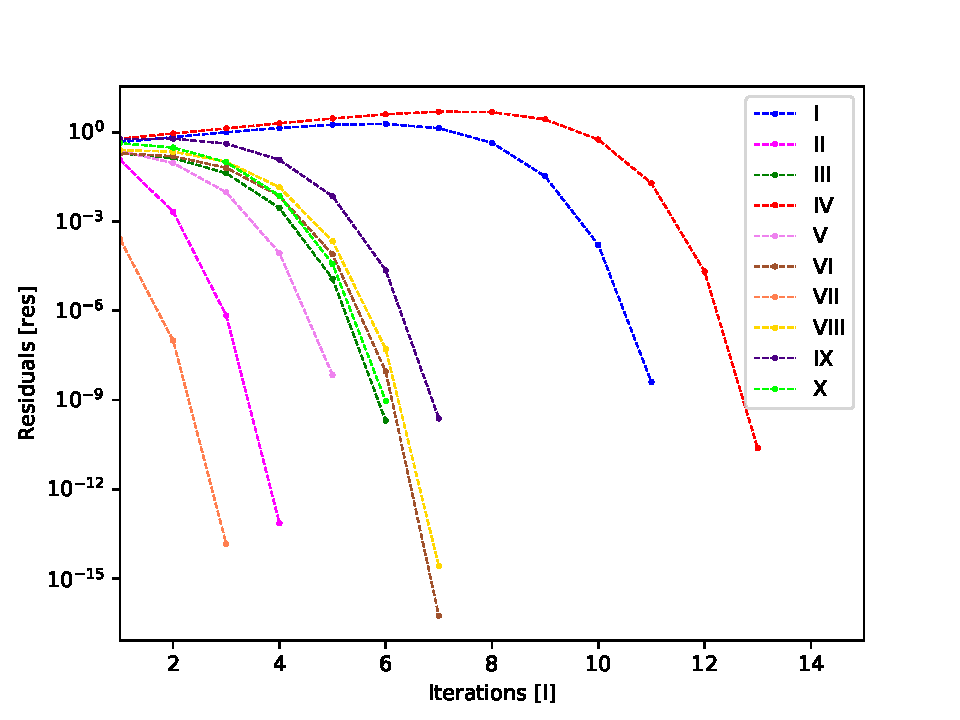
\includegraphics[width=0.85\textwidth]{figure/Newton_Test.pdf}
		\caption{Residual versus number of Newton iterations for the manufactured functions using linear approximation.}
		\label{fig:residuals_newton}
		\end{center}
	\end{figure}


Newton's method was then tested for randomly generated $a_i$ and $b_i$. For these tests, the  $\delta$ was selected randomly between $0$ and $f(0)$ and $x_0=0$ was used as initial estimate. However, $x_0=0$ is a bad estimate in most cases. Smaller the minimum $a_i$, steeper is the shape of the function and a Newton step from $x_0 = 0$ can result in divergence in a very small number of iterations. Also as  the minimum $b_i$ gets smaller, the rightmost vertical asymptote gets closer to the estimate leading to convergence issues.

\subsection*{(c) Newton's method with rational approximation}	
	The function $f(x)$ can be better approximated through a rational function $g(x)$ defined as follows:
	\begin{equation}
		g(x) = \frac{A}{B+x}
	\end{equation}
	Parameters $A$ and $B$ for iteration $n+1$  can be computed from the value of the function and its derivative at iteration $n$. If $x_n$ is the estimate of the root at iteration $n$, then the parameters  $A$ and $B$ can be estimated from the following equations:
	\begin{align}
		g(x_n) = f(x_n) \\
		g'(x_n) = f'(x_n) \\
	\end{align}
	
	Solving the above equations for  $A_n$ and $B_n$ gives:
	\begin{align}
		A_n &= \frac{\left(\sum_{i=1}^N \frac{a_i^2}{(b_i^2+x_n)^2}\right)^2}{2\left(\sum_{i=1}^N \frac{a_i^2}{(b_i^2+x_n)^3}\right)} \\
		B_n &= \frac{\left(\sum_{i=1}^N \frac{a_i^2}{(b_i^2+x_n)^2}\right)}{2\left(\sum_{i=1}^N \frac{a_i^2}{(b_i^2+x_n)^3}\right)} - x_n
	\end{align}
	where the subscript $n$ highlights the fact that $A$ and $B$ are calculated at iteration $n$ and change at each iteration.
	
	The estimate of root at iteration $n+1$ is then the following:
	\begin{equation}
		x_{n+1} = \frac{A_n}{\delta} - B_n
	\end{equation}
	
\subsection*{(d) Implementation of Newton's method with rational approximation}
	Newton's method with rational approximation was implemented and tested for the same ``manufactured" functions  as the Newton's method with linear approximation using the same $delta$ and initial guess $x_0$. This allowed a fair comparison of the two methods and also served as a test to verify the implementation since the results could be compared with the a-priori known results (from solving manufactured functions). Rational approximation shows much better convergence rate when compared to the linear approximation since it approximates the original function much closer than the linear approximation. Also, the method converges in  less than ten iterations as compared to the linear approximation which can take thousands of iterations to converge depending on the values of $a_i$ and $b_i$. Figure~\ref{fig:residuals_newton_modified} shows the residuals versus the number of Newton iterations for the rational function case.
	\begin{figure}[htbp]
		\begin{center}
		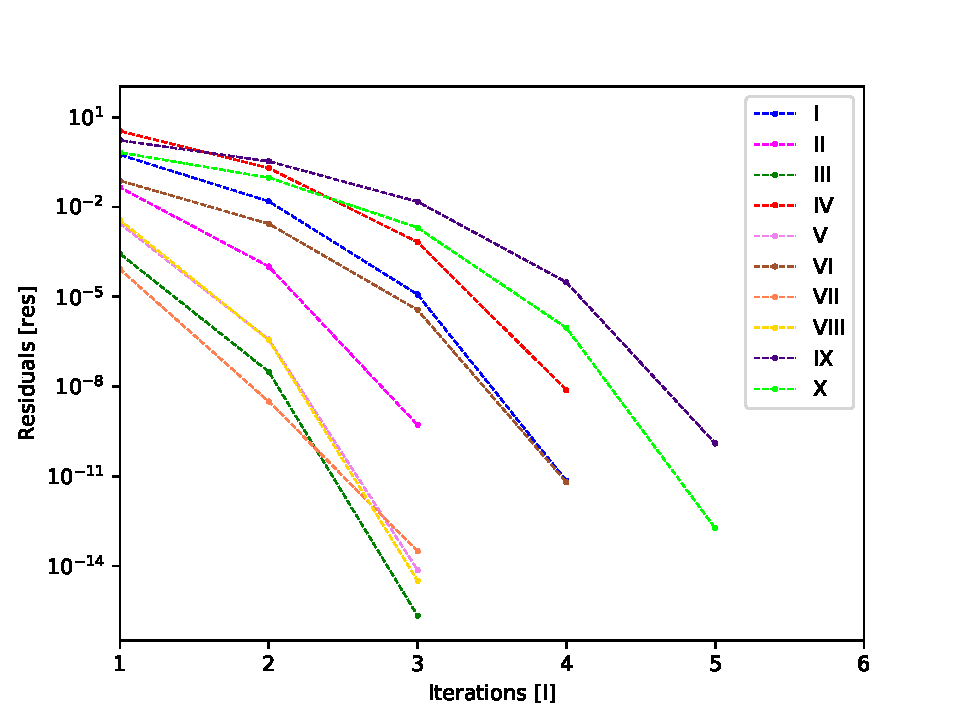
\includegraphics[width=0.85\textwidth]{figure/Newton_Modified_Test.pdf}
		\caption{Residual versus number of Newton iterations for the manufactured functions using rational approximation.}
		\label{fig:residuals_newton_modified}
		\end{center}
	\end{figure}
	
	Like the linear approximation, the convergence of rational approximation also depends on the initial guess and the values of parameters $a_i$ and $b_i$. Since the minimum $a_i$ and minimum $b_i$ are the dominant factors affecting the shape of the function, the asymptotes and subsequently the root, the following initial guess approximation can theoretically be used:
	\begin{equation}
		x_0 = \frac{\min_i (a_i)^2}{\delta} - {\min_i (b_i)^2}
	\end{equation}
	However, the method did not work when implemented and has therefore not been used in the codes. The method was also tested for randomly generated $a_i$ and $b_i$. For these tests, the  $\delta$ was selected randomly between $0$ and $f(0)$ and $x_0=0$ was used as initial estimate. $x_0 = 0$ is still a bad initial guess and while the rational approximation resulted in convergence more often than the linear approximation, it did fail to converge numerous times. However, even when it failed to converge, the residuals and errors were still less than the linear approximation. A comparison of the two methods has been shown in figures~\ref{fig:comparison1} and \ref{fig:comparison1}. The comparison shows that both the methods converge quadratically when the initial guess is close to the correct solution. However, the linear method might not show quadratic convergence if the initial estimate is not close enough. The rational function performs much better in this context and shows almost quadratic convergence.
	
\textbf{Note:} Marcos Machado and myself worked together on this assignment and therefore the codes and plots are common.
	
	\begin{figure}
		\centering
		\begin{subfigure}[b]{.45\linewidth}
			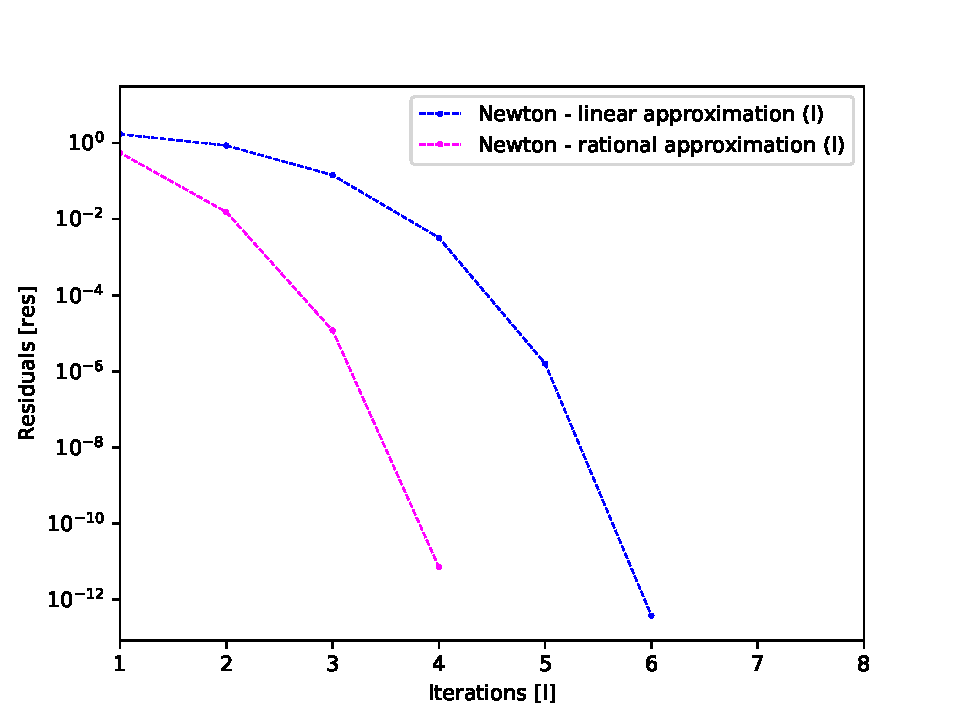
\includegraphics[width=\linewidth]{figure/1.pdf}
			\caption{Case 1}
		\end{subfigure}
		\begin{subfigure}[b]{.45\linewidth}
			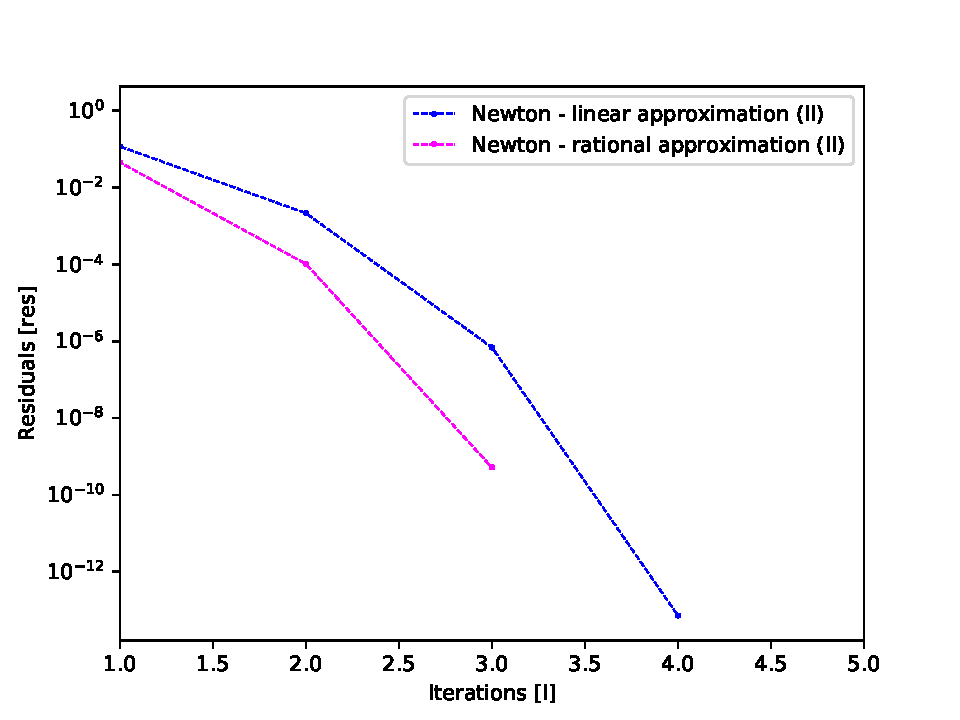
\includegraphics[width=\linewidth]{figure/2.pdf}
			\caption{Case 2}
		\end{subfigure}
		

		\begin{subfigure}[b]{.45\linewidth}
			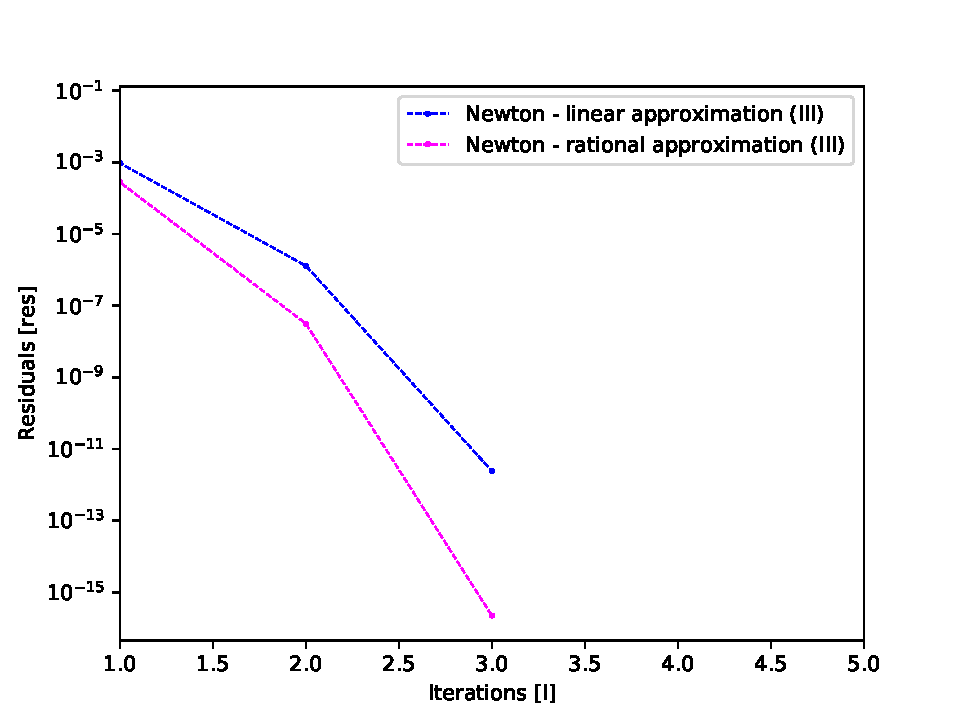
\includegraphics[width=\linewidth]{figure/3.pdf}
			\caption{Case 3}
		\end{subfigure}
		\begin{subfigure}[b]{.45\linewidth}
			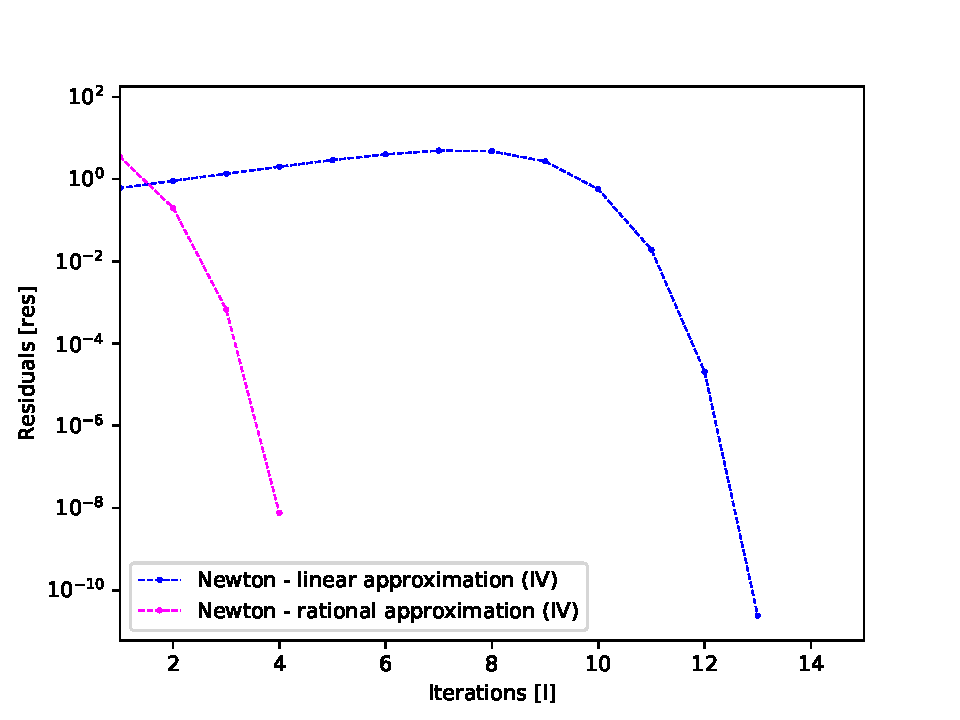
\includegraphics[width=\linewidth]{figure/4.pdf}
			\caption{Case 4}
		\end{subfigure}
		
		\begin{subfigure}[b]{.45\linewidth}
			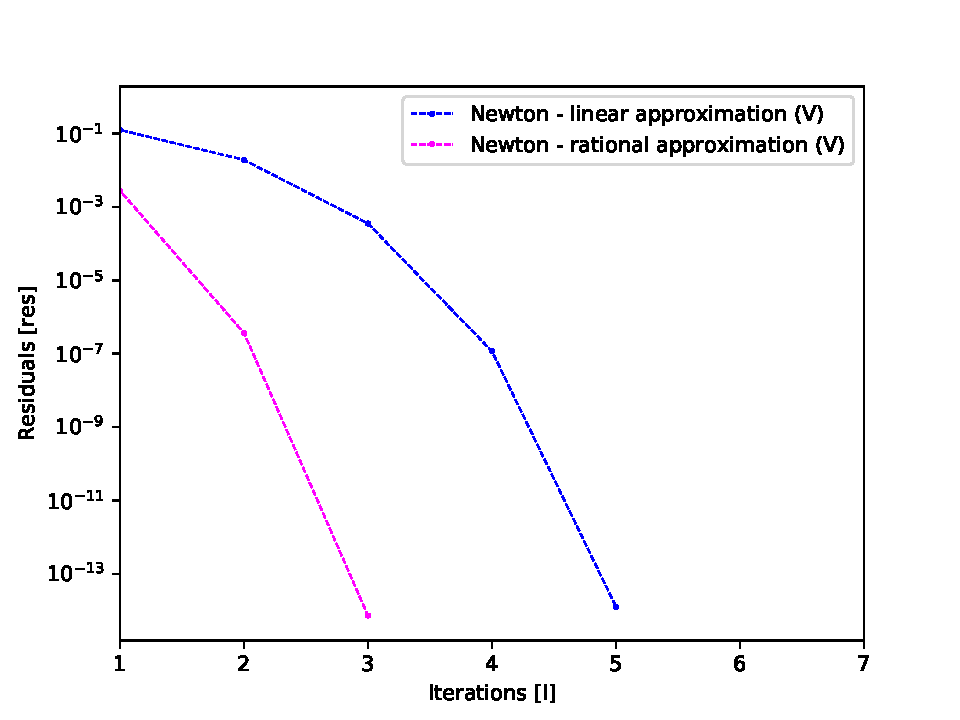
\includegraphics[width=\linewidth]{figure/5.pdf}
			\caption{Case 5}
		\end{subfigure}
		\begin{subfigure}[b]{.45\linewidth}
			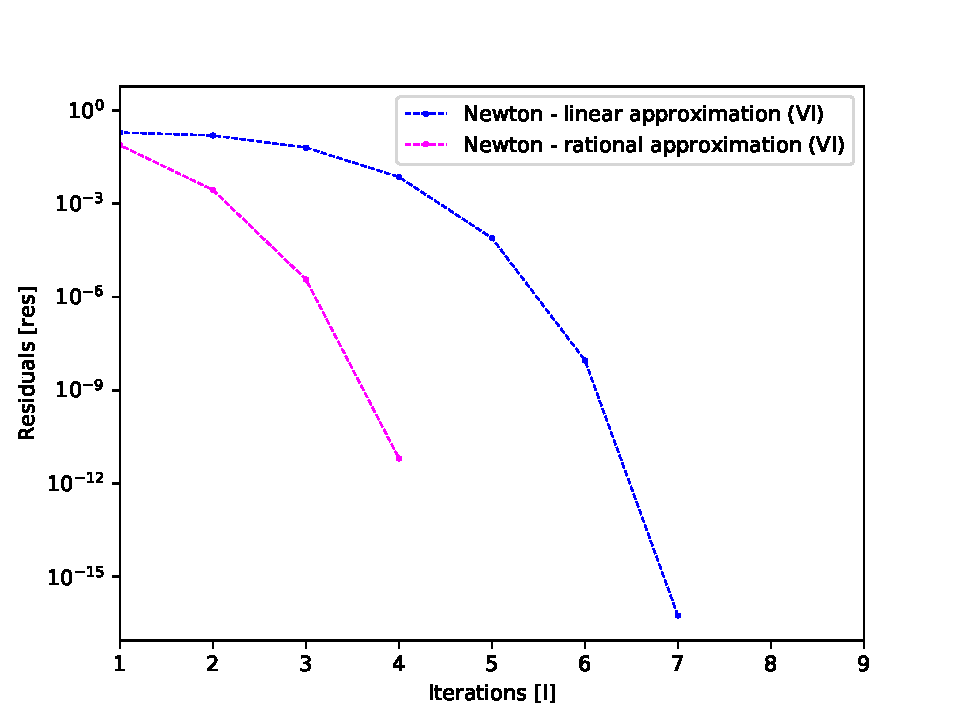
\includegraphics[width=\linewidth]{figure/6.pdf}
			\caption{Case 6}
		\end{subfigure}
		\caption{Comparison of linear and rational approximations for the manufactured functions.}
		\label{fig:comparison1}
	\end{figure}
	\begin{figure}
		\centering
		\begin{subfigure}[b]{.45\linewidth}
			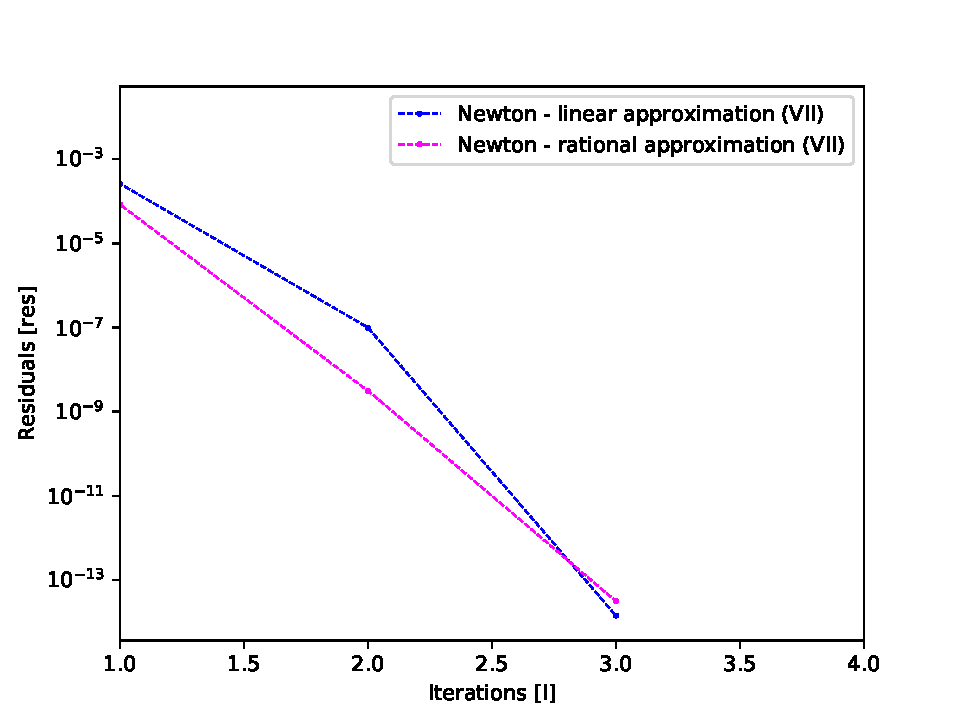
\includegraphics[width=\linewidth]{figure/7.pdf}
			\caption{Case 7}
		\end{subfigure}
		\begin{subfigure}[b]{.45\linewidth}
			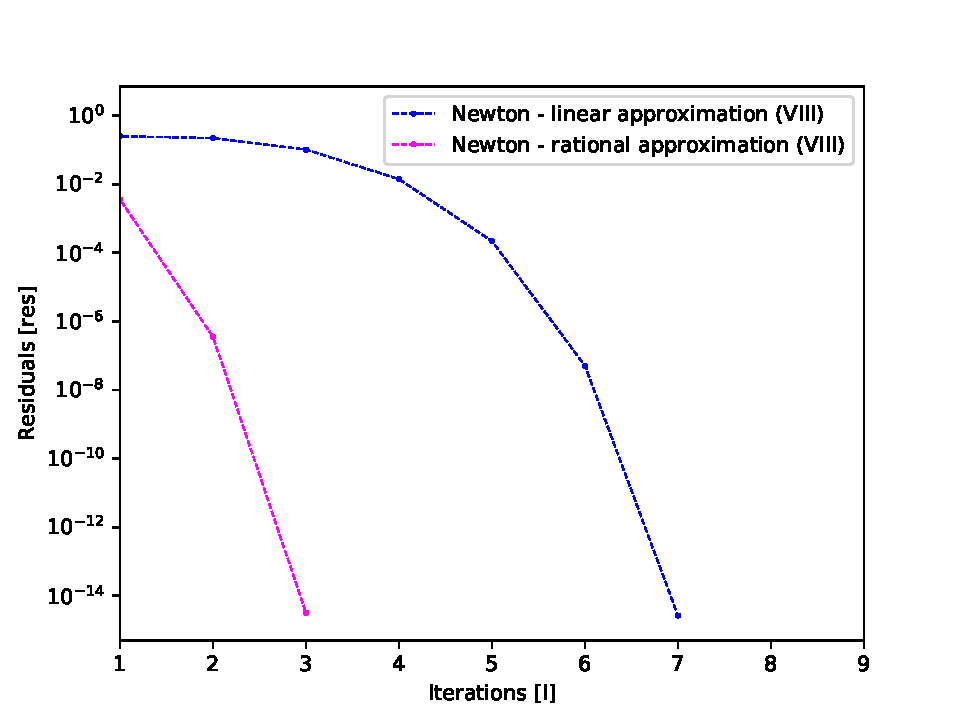
\includegraphics[width=\linewidth]{figure/8.pdf}
			\caption{Case 8}
		\end{subfigure}
		

		\begin{subfigure}[b]{.45\linewidth}
			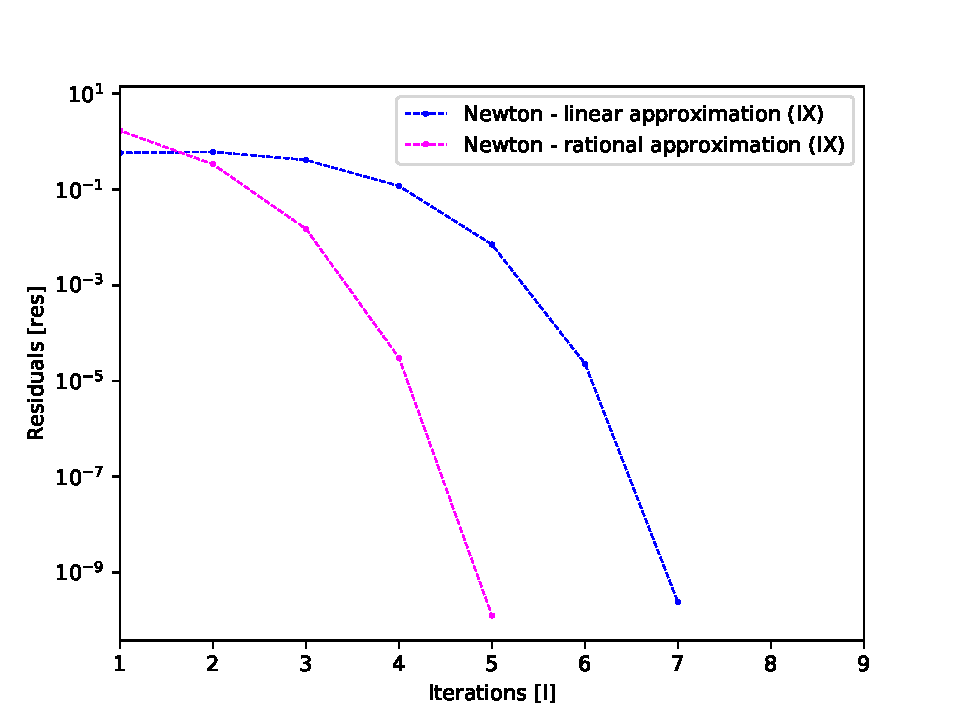
\includegraphics[width=\linewidth]{figure/9.pdf}
			\caption{Case 9}
		\end{subfigure}
		\begin{subfigure}[b]{.45\linewidth}
			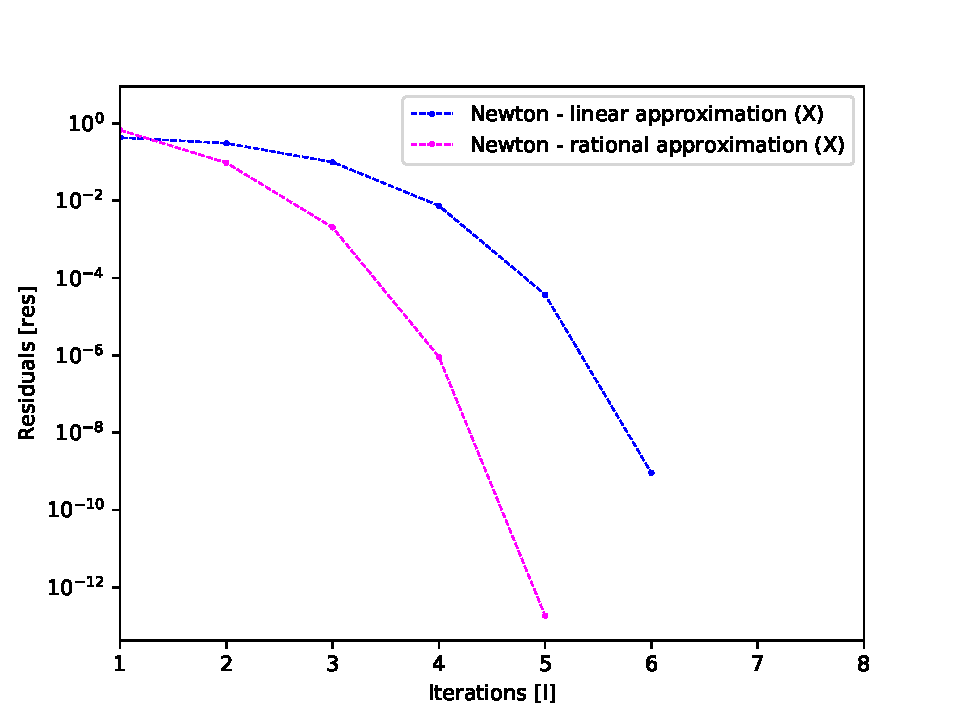
\includegraphics[width=\linewidth]{figure/10.pdf}
			\caption{Case 10}
		\end{subfigure}
		\caption{Comparison of linear and rational approximations for the manufactured functions.}
		\label{fig:comparison2}
	\end{figure}
	
\end{document}
